\subsubsection {Hypothesis Testing}
From linear regression, we can get t-statistics for different conditions(task on/off, gain, loss, d
istance).For each condition, we will have a 3D t-statistics matrix. For visualization, we first ad
ded mask based the mean voxel and the histogram. We set a boolean mask which takes larger than 375
. Also we used smooth function and better color txt to generate a better image. Then we plotted t
he t statistics map for gain/loss. 
\begin{figure}[H]
\begin{subfigure}{.5\textwidth}
  \centering
  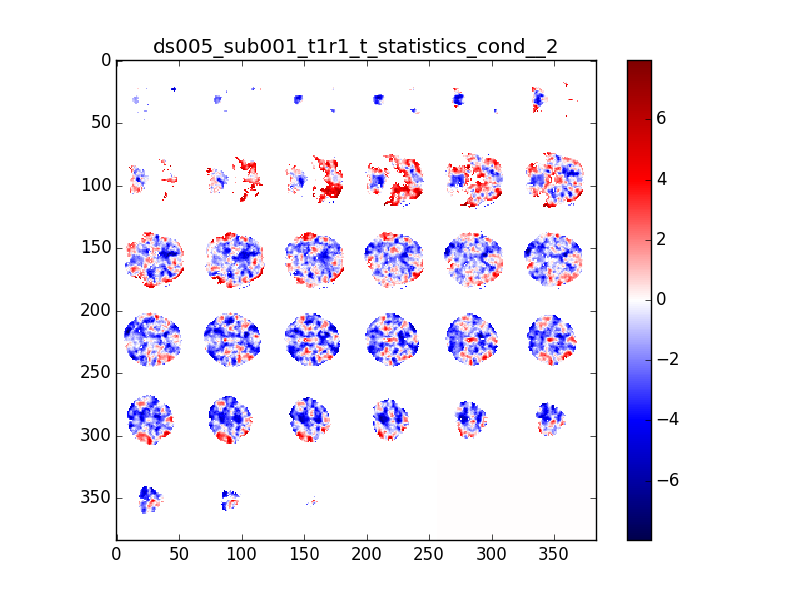
\includegraphics[width=.9\linewidth]{../fig/t_test/ds005_sub001_t1r1_t-test_cond2.png}
  \caption{Gain}
  \label{fig:sfig1}
\end{subfigure}%
\begin{subfigure}{.5\textwidth}
  \centering
  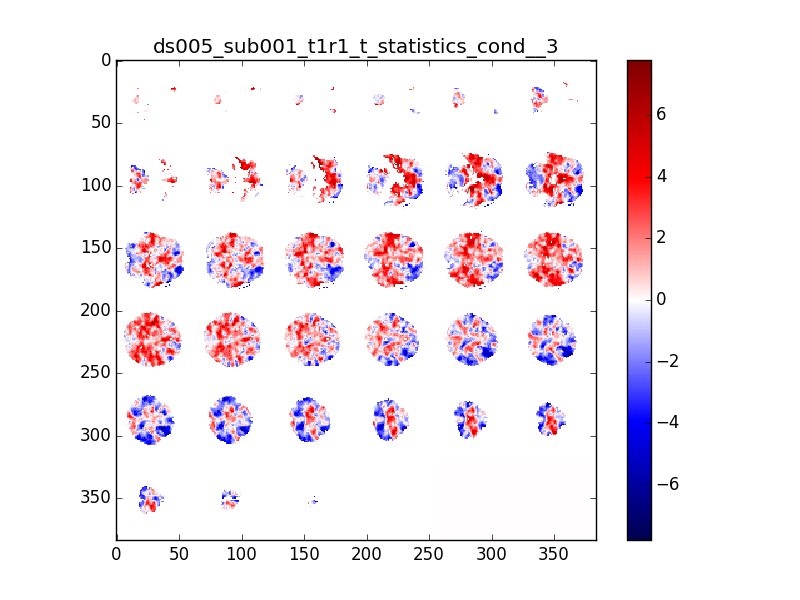
\includegraphics[width=.9\linewidth]{../fig/t_test/ds005_sub001_t1r1_t-test_cond3.png}
  \caption{Loss}
  \label{fig:sfig2}
\end{subfigure}
\caption{t statistics map for gain/loss (subject1)}
\label{fig:fig}
\end{figure}

\begin{figure}[H]
\begin{subfigure}{.5\textwidth}
  \centering
  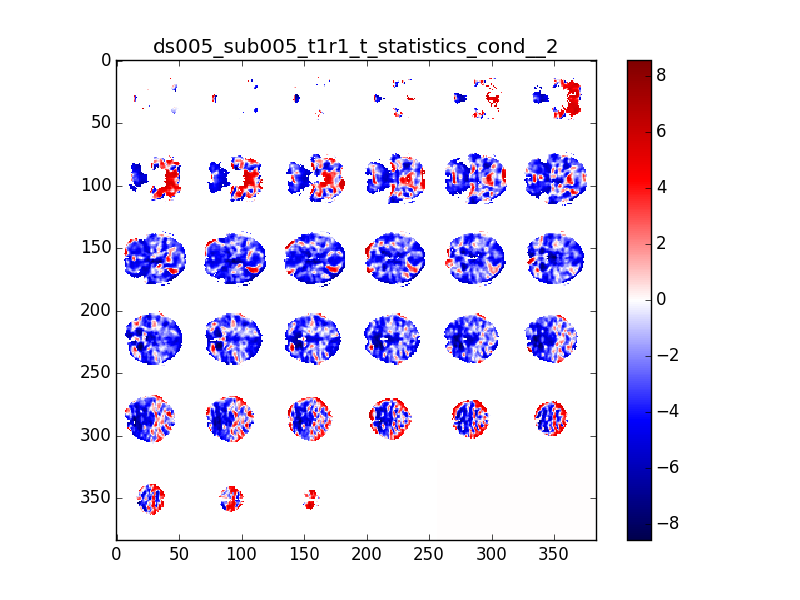
\includegraphics[width=.9\linewidth]{../fig/t_test/ds005_sub005_t1r1_t-test_cond2.png}
  \caption{Gain}
  \label{fig:sfig1}
\end{subfigure}%
\begin{subfigure}{.5\textwidth}
  \centering
  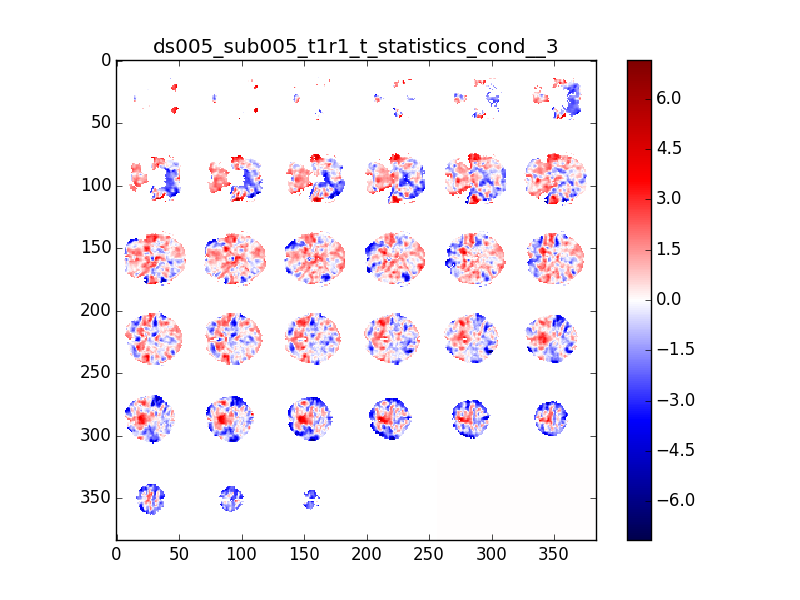
\includegraphics[width=.9\linewidth]{../fig/t_test/ds005_sub005_t1r1_t-test_cond3.png}
  \caption{Loss}
  \label{fig:sfig2}
\end{subfigure}
\caption{t statistics map for gain/loss (subject5)}
\label{fig:fig}
\end{figure}
\noindent
The larger the t-statistics, the more significant. Thus the red spots represents the activa
ted voxels for gain and loss. For subject 1, gain has more activated voxels. However, for su
bject 5, loss has more activated voxels.

